\section{Hardware connection}

Figure \ref{fig:sch} shows the schematic diagram of our robot, power cables are not shown. We made several change to the previous proposal due to some realistic conditions. We first remove UWB and GPS from the previous proposal. This is because we already included enough number of functions, while GPS and UWB will not significantly affect the result of our robot. Secondly, Instead of employing 4 Degree of Freedom(Dof), we finally decided to use three Dofs bacause too many Dofs are not necessary to achieve our tasks. Finally, we used one camera instead of two cameras, and remove the unnecessary microphone.
\begin{figure}[H]
    \centering
    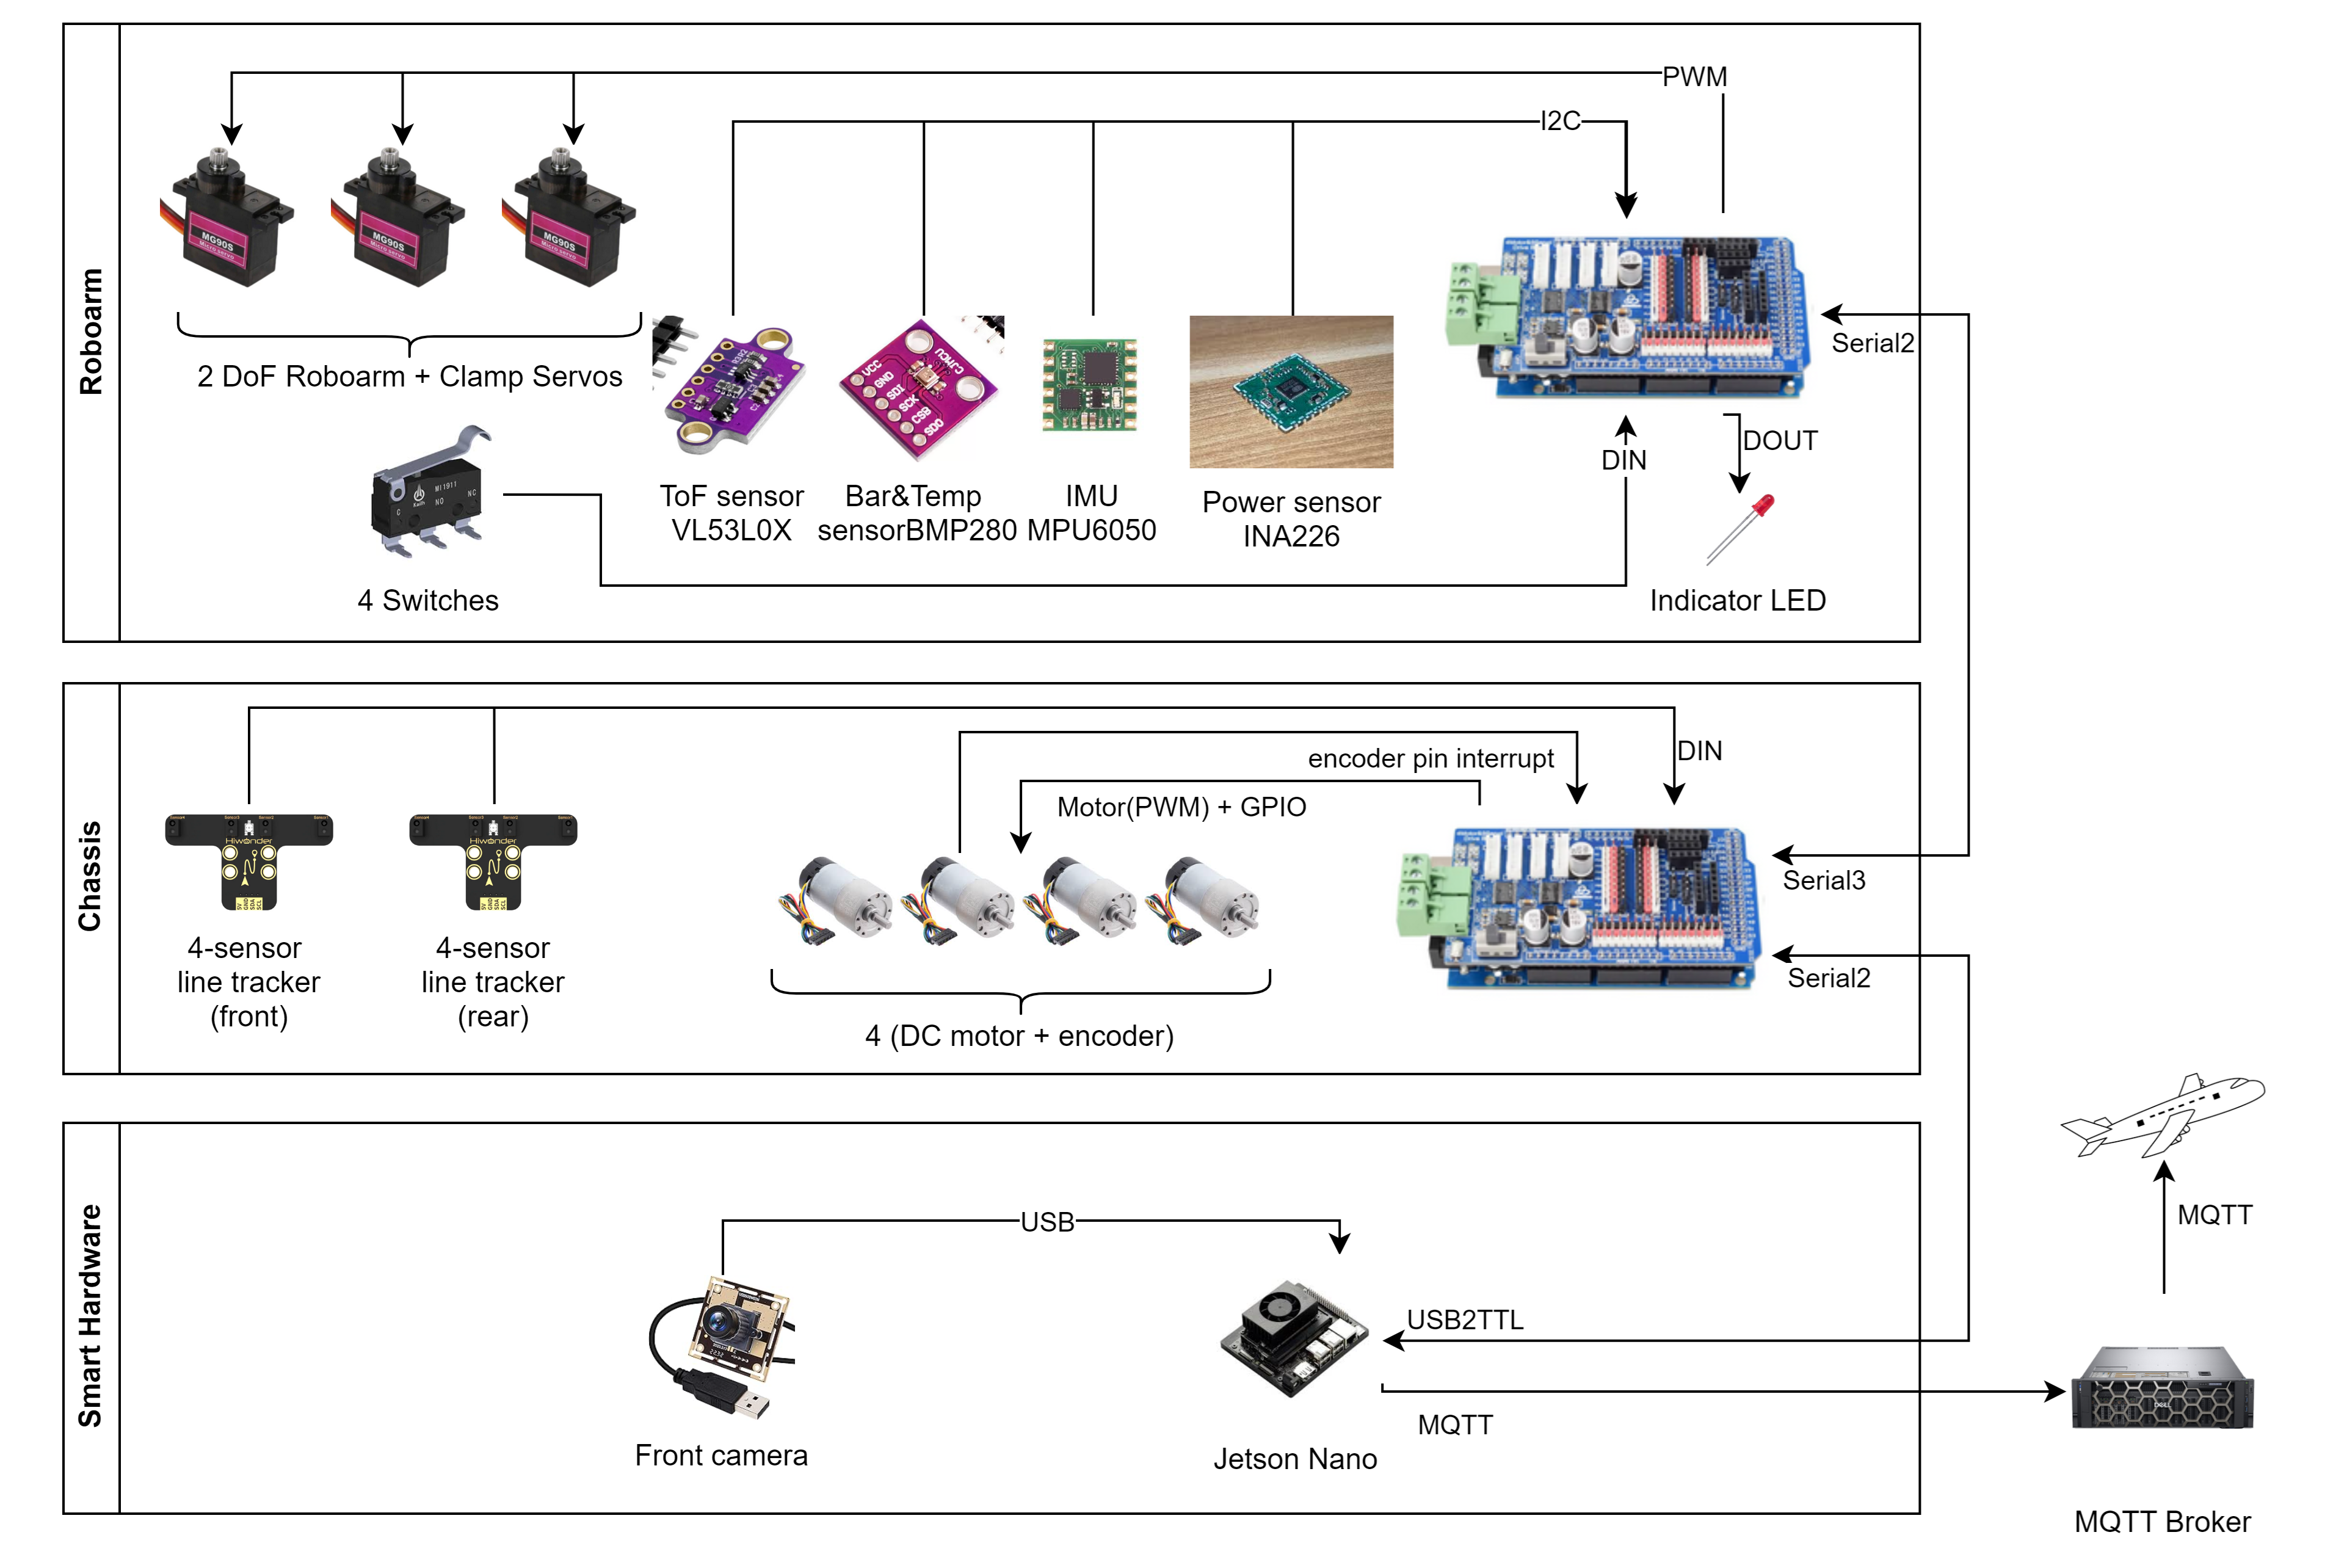
\includegraphics[width=\linewidth]{asset/elec3848_sch.png}
    \caption{
    Schematic diagram of the robot. Chassis board is connected to chassis movement related hardware
    (2 line trackers and 4 DC motors), Roboarm board is connected to roboarm and sensor related hardware
    (3 PWM servos, micro switches, ToF, BMP, IMU, and INA sensors). The Jetson is only connected to the 
    chassis board through TTL serial and the two Arduino boards are inter-connected with serial port.
    }
    \label{fig:sch}
\end{figure}




